% vim: set spell spelllang=es syntax=tex :

\section{Fútbol de robots}

La \emph{RoboCup}\cite{robocupHist} (del inglés \emph{Robot World Cup}) es una
competencia internacional celebrada desde 1997, donde equipos de robots juegan
una versión simplificada del fútbol. Su finalidad es la de ofrecer un ambiente
controlado donde poner a prueba los avances en distintas áreas de conocimiento
como la inteligencia artificial, visión por computadora y robótica. Existen
cinco ligas distintas cuyas características varían desde la simulación del
ambiente y de los robots, hasta robots humanoides con visión local. De éstas, la
más antigua es la liga de tamaño pequeño (\emph{SSL}, del inglés \emph{Small
Size League}).

Nota de OSO: Se puede agregar info detallada de cada una de las ligas

Un partido de la \emph{SSL} enfrenta a dos equipos de seis robots, que deben
tener un tamaño menor que un cilindro de 9$cm$ de radio y 15$cm$ de
alto\cite{sslrules2015}. Los robots tienen capacidad de procesamiento reducida,
y cada equipo cuenta con una computadora fuera del campo de juego, a la cual se
delega la toma de decisiones. Estas computadoras perciben el ambiente a través
de un sistema de visión global centralizado compartido. Se utiliza un conjunto
de cámaras, montadas sobre distintas áreas del campo de juego y conectadas a una
computadora donde se ejecuta el sistema de visión. El sistema detecta la
posición y orientación de cada uno de los robots y la posición de la pelota, y
reporta esta información a las computadoras que controlan los equipos.

Para que el sistema de visión pueda identificar a cada robot, cada uno tiene
sobre su parte superior cinco parches de colores (Fig. \ref{sistemaVG}). El
parche que se encuentra en el centro indica el color del equipo del robot, y los
cuatro restantes sirven para identificar al robot dentro del equipo y para
conocer la orientación que lleva en cada momento. La pelota es de un color
uniforme y distinto al de los parches de los robots; normalmente, naranja, ya
que este color contrasta fácilmente con el verde de la cancha.

\begin{figure}[!h]

	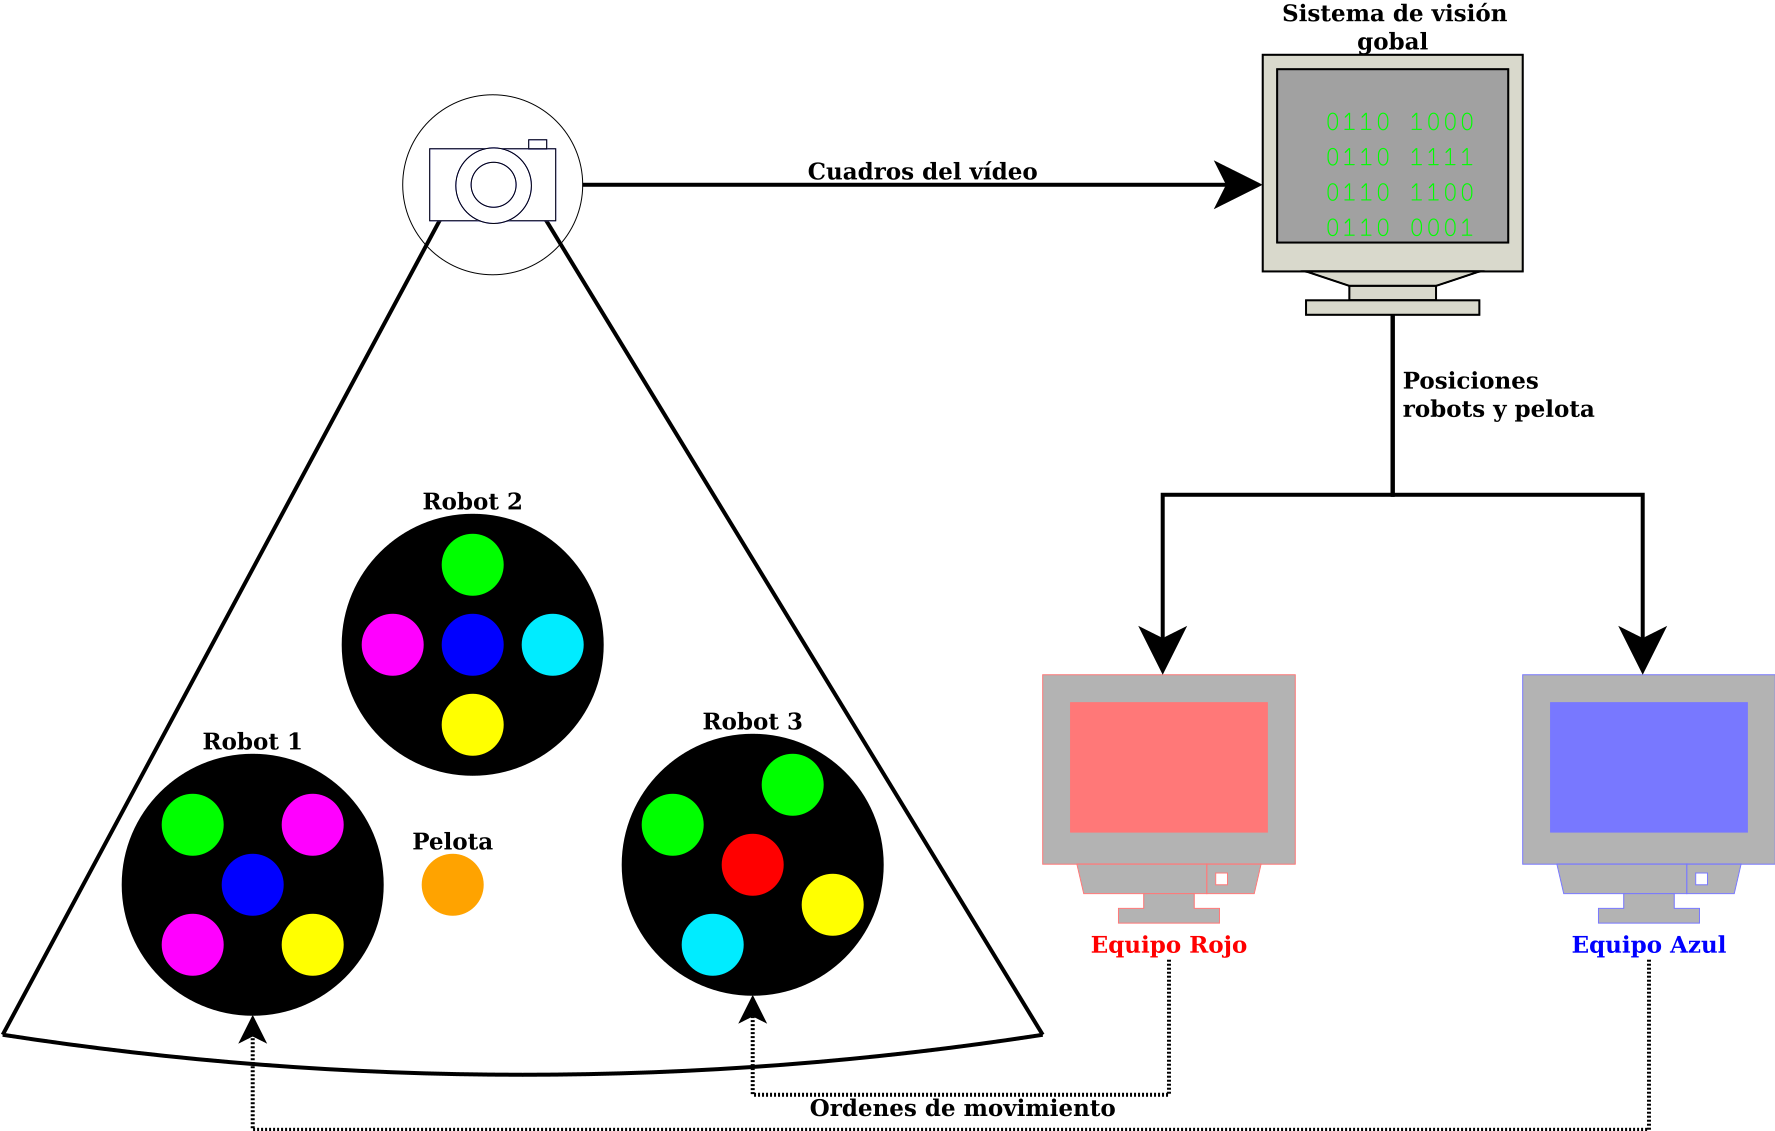
\includegraphics[width=\textwidth]{img/sistemaVG.pdf}

	\caption{Estructura de comunicación del sistema de visión global en
	fútbol de robots de la \emph{SSL}.}

	\label{sistemaVG}

\end{figure}

El uso de este sistema centralizado permite a los participantes abstraerse de
los problemas de la visión por computadora y enfocarse en la estrategia del
juego. Además, permite que las tareas de calibración y montaje de las cámaras se
realicen una sola vez para cada campo de juego, en vez de para cada partido.

Originalmente el tamaño de la cancha era de 4,9$m\times$3,4$m$, lo que permitía
que todo el campo de juego fuera observado con una sola cámara. Luego se optó
por dos tipos de canchas en los partidos de la \emph{SSL}: las canchas de tamaño
simple, con un tamaño de 6,05$m\times$4,05$m$ para las cuales se utilizan dos
cámaras, una sobre cada media cancha, y las de tamaño doble, con un tamaño de
8,09$m\times$6,05$m$, que utilizan cuatro cámaras, una por cada mitad de cada
media cancha (Fig. \ref{FALTA}). Desde el año 2015, las canchas de tamaño doble
son las utilizadas de forma predeterminada\cite{sslrules2015}. Con este cambio
se espera permitir la exploración de nuevas tácticas por parte de los equipos,
ya que una mayor área de juego permite a los robots movimientos de mayor
amplitud y variedad.

\begin{figure}[!h]

	
\includegraphics[width=\textwidth]{img/FALTA.png}

	\caption{Dimensiones y área de cobertura de las cámaras en la liga
	\emph{SSL}, en competencias a) anteriores a 2015; b) año 2015 y
	posteriores.}

	\label{FALTA}

\end{figure}

Sin embargo, como consecuencia, en las canchas de tamaño doble, el sistema de
visión debe procesar cuatro veces más información que en las canchas originales;
lo que da lugar a un problema. En efecto, el fútbol de robots se desarrolla en
un contexto de tiempo real, ya que el ciclo completo de procesamiento de
información debe cumplirse en un plazo máximo para poder alcanzar los objetivos.
El servidor debe procesar cada cuadro para entregar la información de posición y
velocidad de cada elemento en el campo de juego a las computadoras coordinadoras
de los equipos; y éstas deben tomar una decisión y comunicarla a los robots,
todo dentro de un tiempo de respuesta razonable para el progreso de la
aplicación.

Los parámetros de calidad de este tipo de sistema son, normalmente:

\begin{itemize}

	\item 	tasa de aciertos en la detección de objetos;

	\item 	precisión en la posición y orientación de los aciertos en la
		detección de objetos;

	\item 	precisión en la posición y orientación de los robots y pelota;

	\item 	cuadros por segundo (\emph{FPS}, del inglés \emph{Frames Per
		Second}) procesados;

	\item 	y máximo tiempo de espera del cuadro (tiempo desde la creación
		del cuadro hasta la entrega de la información extraída).

\end{itemize}

Duplicar la cantidad de información que se debe procesar impacta negativamente
en el rendimiento de estos sistemas, debido a que se reducen los cuadros por
segundo procesados y se incrementa el tiempo de espera del cuadro. Para aumentar
el rendimiento de estos sistemas es necesario implementar soluciones paralelas
que aprovechen las múltiples unidades de procesamiento de las arquitecturas de
cómputo actuales.
